% REV00 Tue 04 May 2021 13:55:16 WIB
% START Tue 04 May 2021 13:55:16 WIB

\chapter{A RESPECTED FRIEND IN A NEW ASPECT}

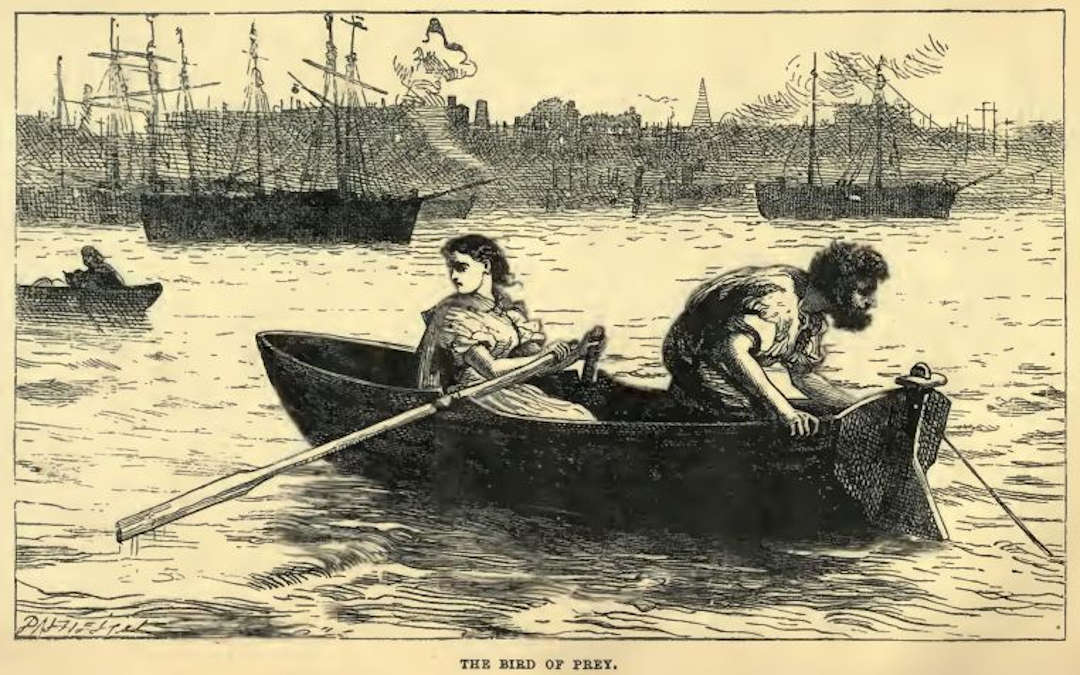
\includegraphics[scale=2.3]{01-01-01}

In the evening of this same foggy day when the yellow window-blind of
Pubsey and Co. was drawn down upon the day’s work, Riah the Jew once
more came forth into Saint Mary Axe. But this time he carried no bag,
and was not bound on his master’s affairs. He passed over London Bridge,
and returned to the Middlesex shore by that of Westminster, and so, ever
wading through the fog, waded to the doorstep of the dolls’ dressmaker.

Miss Wren expected him. He could see her through the window by the light
of her low fire--carefully banked up with damp cinders that it might
last the longer and waste the less when she was out--sitting waiting
for him in her bonnet. His tap at the glass roused her from the musing
solitude in which she sat, and she came to the door to open it; aiding
her steps with a little crutch-stick.

‘Good evening, godmother!’ said Miss Jenny Wren.

The old man laughed, and gave her his arm to lean on.

‘Won’t you come in and warm yourself, godmother?’ asked Miss Jenny Wren.

‘Not if you are ready, Cinderella, my dear.’

‘Well!’ exclaimed Miss Wren, delighted. ‘Now you ARE a clever old boy!
If we gave prizes at this establishment (but we only keep blanks), you
should have the first silver medal, for taking me up so quick.’ As she
spake thus, Miss Wren removed the key of the house-door from the keyhole
and put it in her pocket, and then bustlingly closed the door, and tried
it as they both stood on the step. Satisfied that her dwelling was safe,
she drew one hand through the old man’s arm and prepared to ply her
crutch-stick with the other. But the key was an instrument of such
gigantic proportions, that before they started Riah proposed to carry
it.

‘No, no, no! I’ll carry it myself,’ returned Miss Wren. ‘I’m awfully
lopsided, you know, and stowed down in my pocket it’ll trim the ship. To
let you into a secret, godmother, I wear my pocket on my high side, o’
purpose.’

With that they began their plodding through the fog.

‘Yes, it was truly sharp of you, godmother,’ resumed Miss Wren with
great approbation, ‘to understand me. But, you see, you ARE so like the
fairy godmother in the bright little books! You look so unlike the rest
of people, and so much as if you had changed yourself into that shape,
just this moment, with some benevolent object. Boh!’ cried Miss Jenny,
putting her face close to the old man’s. ‘I can see your features,
godmother, behind the beard.’

‘Does the fancy go to my changing other objects too, Jenny?’

‘Ah! That it does! If you’d only borrow my stick and tap this piece of
pavement--this dirty stone that my foot taps--it would start up a coach
and six. I say! Let’s believe so!’

‘With all my heart,’ replied the good old man.

‘And I’ll tell you what I must ask you to do, godmother. I must ask you
to be so kind as give my child a tap, and change him altogether. O my
child has been such a bad, bad child of late! It worries me nearly
out of my wits. Not done a stroke of work these ten days. Has had the
horrors, too, and fancied that four copper-coloured men in red wanted to
throw him into a fiery furnace.’

‘But that’s dangerous, Jenny.’

‘Dangerous, godmother? My child is always dangerous, more or less. He
might’--here the little creature glanced back over her shoulder at the
sky--‘be setting the house on fire at this present moment. I don’t know
who would have a child, for my part! It’s no use shaking him. I have
shaken him till I have made myself giddy. “Why don’t you mind your
Commandments and honour your parent, you naughty old boy?” I said to him
all the time. But he only whimpered and stared at me.’

‘What shall be changed, after him?’ asked Riah in a compassionately
playful voice.

‘Upon my word, godmother, I am afraid I must be selfish next, and get
you to set me right in the back and the legs. It’s a little thing to you
with your power, godmother, but it’s a great deal to poor weak aching
me.’

There was no querulous complaining in the words, but they were not the
less touching for that.

‘And then?’

‘Yes, and then--YOU know, godmother. We’ll both jump up into the coach
and six and go to Lizzie. This reminds me, godmother, to ask you a
serious question. You are as wise as wise can be (having been brought
up by the fairies), and you can tell me this: Is it better to have had a
good thing and lost it, or never to have had it?’

‘Explain, god-daughter.’

‘I feel so much more solitary and helpless without Lizzie now, than I
used to feel before I knew her.’ (Tears were in her eyes as she said
so.)

‘Some beloved companionship fades out of most lives, my dear,’ said the
Jew,--‘that of a wife, and a fair daughter, and a son of promise, has
faded out of my own life--but the happiness was.’

‘Ah!’ said Miss Wren thoughtfully, by no means convinced, and chopping
the exclamation with that sharp little hatchet of hers; ‘then I tell you
what change I think you had better begin with, godmother. You had better
change Is into Was and Was into Is, and keep them so.’

‘Would that suit your case? Would you not be always in pain then?’ asked
the old man tenderly.

‘Right!’ exclaimed Miss Wren with another chop. ‘You have changed me
wiser, godmother.--Not,’ she added with the quaint hitch of her chin and
eyes, ‘that you need be a very wonderful godmother to do that deed.’

Thus conversing, and having crossed Westminster Bridge, they traversed
the ground that Riah had lately traversed, and new ground likewise; for,
when they had recrossed the Thames by way of London Bridge, they struck
down by the river and held their still foggier course that way.

But previously, as they were going along, Jenny twisted her venerable
friend aside to a brilliantly-lighted toy-shop window, and said: ‘Now
look at ‘em! All my work!’

This referred to a dazzling semicircle of dolls in all the colours of
the rainbow, who were dressed for presentation at court, for going to
balls, for going out driving, for going out on horseback, for going out
walking, for going to get married, for going to help other dolls to get
married, for all the gay events of life.

‘Pretty, pretty, pretty!’ said the old man with a clap of his hands.
‘Most elegant taste!’

‘Glad you like ‘em,’ returned Miss Wren, loftily. ‘But the fun is,
godmother, how I make the great ladies try my dresses on. Though it’s
the hardest part of my business, and would be, even if my back were not
bad and my legs queer.’

He looked at her as not understanding what she said.

‘Bless you, godmother,’ said Miss Wren, ‘I have to scud about town at
all hours. If it was only sitting at my bench, cutting out and sewing,
it would be comparatively easy work; but it’s the trying-on by the great
ladies that takes it out of me.’

‘How, the trying-on?’ asked Riah.

‘What a mooney godmother you are, after all!’ returned Miss Wren. ‘Look
here. There’s a Drawing Room, or a grand day in the Park, or a Show, or
a Fete, or what you like. Very well. I squeeze among the crowd, and I
look about me. When I see a great lady very suitable for my business, I
say “You’ll do, my dear!” and I take particular notice of her, and run
home and cut her out and baste her. Then another day, I come scudding
back again to try on, and then I take particular notice of her again.
Sometimes she plainly seems to say, ‘How that little creature is
staring!’ and sometimes likes it and sometimes don’t, but much more
often yes than no. All the time I am only saying to myself, “I must
hollow out a bit here; I must slope away there;” and I am making a
perfect slave of her, with making her try on my doll’s dress. Evening
parties are severer work for me, because there’s only a doorway for a
full view, and what with hobbling among the wheels of the carriages
and the legs of the horses, I fully expect to be run over some night.
However, there I have ‘em, just the same. When they go bobbing into the
hall from the carriage, and catch a glimpse of my little physiognomy
poked out from behind a policeman’s cape in the rain, I dare say they
think I am wondering and admiring with all my eyes and heart, but they
little think they’re only working for my dolls! There was Lady Belinda
Whitrose. I made her do double duty in one night. I said when she came
out of the carriage, “YOU’ll do, my dear!” and I ran straight home and
cut her out and basted her. Back I came again, and waited behind the men
that called the carriages. Very bad night too. At last, “Lady Belinda
Whitrose’s carriage! Lady Belinda Whitrose coming down!” And I made her
try on--oh! and take pains about it too--before she got seated. That’s
Lady Belinda hanging up by the waist, much too near the gaslight for a
wax one, with her toes turned in.’

When they had plodded on for some time nigh the river, Riah asked
the way to a certain tavern called the Six Jolly Fellowship Porters.
Following the directions he received, they arrived, after two or three
puzzled stoppages for consideration, and some uncertain looking about
them, at the door of Miss Abbey Potterson’s dominions. A peep through
the glass portion of the door revealed to them the glories of the bar,
and Miss Abbey herself seated in state on her snug throne, reading the
newspaper. To whom, with deference, they presented themselves.

Taking her eyes off her newspaper, and pausing with a suspended
expression of countenance, as if she must finish the paragraph in hand
before undertaking any other business whatever, Miss Abbey demanded,
with some slight asperity: ‘Now then, what’s for you?’

‘Could we see Miss Potterson?’ asked the old man, uncovering his head.

‘You not only could, but you can and you do,’ replied the hostess.

‘Might we speak with you, madam?’

By this time Miss Abbey’s eyes had possessed themselves of the small
figure of Miss Jenny Wren. For the closer observation of which, Miss
Abbey laid aside her newspaper, rose, and looked over the half-door of
the bar. The crutch-stick seemed to entreat for its owner leave to come
in and rest by the fire; so, Miss Abbey opened the half-door, and said,
as though replying to the crutch-stick:

‘Yes, come in and rest by the fire.’

‘My name is Riah,’ said the old man, with courteous action, ‘and my
avocation is in London city. This, my young companion--’

‘Stop a bit,’ interposed Miss Wren. ‘I’ll give the lady my card.’ She
produced it from her pocket with an air, after struggling with the
gigantic door-key which had got upon the top of it and kept it down.
Miss Abbey, with manifest tokens of astonishment, took the diminutive
document, and found it to run concisely thus:--


		MISS JENNY WREN

	       DOLLS’ DRESSMAKER.

	Dolls attended at their own residences.


‘Lud!’ exclaimed Miss Potterson, staring. And dropped the card.

‘We take the liberty of coming, my young companion and I, madam,’ said
Riah, ‘on behalf of Lizzie Hexam.’

Miss Potterson was stooping to loosen the bonnet-strings of the dolls’
dressmaker. She looked round rather angrily, and said: ‘Lizzie Hexam is
a very proud young woman.’

‘She would be so proud,’ returned Riah, dexterously, ‘to stand well in
your good opinion, that before she quitted London for--’

‘For where, in the name of the Cape of Good Hope?’ asked Miss Potterson,
as though supposing her to have emigrated.

‘For the country,’ was the cautious answer,--‘she made us promise to
come and show you a paper, which she left in our hands for that special
purpose. I am an unserviceable friend of hers, who began to know her
after her departure from this neighbourhood. She has been for some time
living with my young companion, and has been a helpful and a comfortable
friend to her. Much needed, madam,’ he added, in a lower voice. ‘Believe
me; if you knew all, much needed.’

‘I can believe that,’ said Miss Abbey, with a softening glance at the
little creature.

‘And if it’s proud to have a heart that never hardens, and a temper
that never tires, and a touch that never hurts,’ Miss Jenny struck in,
flushed, ‘she is proud. And if it’s not, she is NOT.’

Her set purpose of contradicting Miss Abbey point blank, was so far from
offending that dread authority, as to elicit a gracious smile. ‘You do
right, child,’ said Miss Abbey, ‘to speak well of those who deserve well
of you.’

‘Right or wrong,’ muttered Miss Wren, inaudibly, with a visible hitch of
her chin, ‘I mean to do it, and you may make up your mind to THAT, old
lady.’

‘Here is the paper, madam,’ said the Jew, delivering into Miss
Potterson’s hands the original document drawn up by Rokesmith, and
signed by Riderhood. ‘Will you please to read it?’

‘But first of all,’ said Miss Abbey, ‘--did you ever taste shrub,
child?’

Miss Wren shook her head.

‘Should you like to?’

‘Should if it’s good,’ returned Miss Wren.

‘You shall try. And, if you find it good, I’ll mix some for you with hot
water. Put your poor little feet on the fender. It’s a cold, cold night,
and the fog clings so.’ As Miss Abbey helped her to turn her chair, her
loosened bonnet dropped on the floor. ‘Why, what lovely hair!’ cried
Miss Abbey. ‘And enough to make wigs for all the dolls in the world.
What a quantity!’

‘Call THAT a quantity?’ returned Miss Wren. ‘Poof! What do you say to
the rest of it?’ As she spoke, she untied a band, and the golden stream
fell over herself and over the chair, and flowed down to the ground.
Miss Abbey’s admiration seemed to increase her perplexity. She beckoned
the Jew towards her, as she reached down the shrub-bottle from its
niche, and whispered:

‘Child, or woman?’

‘Child in years,’ was the answer; ‘woman in self-reliance and trial.’

‘You are talking about Me, good people,’ thought Miss Jenny, sitting in
her golden bower, warming her feet. ‘I can’t hear what you say, but I
know your tricks and your manners!’

The shrub, when tasted from a spoon, perfectly harmonizing with Miss
Jenny’s palate, a judicious amount was mixed by Miss Potterson’s skilful
hands, whereof Riah too partook. After this preliminary, Miss Abbey read
the document; and, as often as she raised her eyebrows in so doing,
the watchful Miss Jenny accompanied the action with an expressive and
emphatic sip of the shrub and water.

‘As far as this goes,’ said Miss Abbey Potterson, when she had read it
several times, and thought about it, ‘it proves (what didn’t much need
proving) that Rogue Riderhood is a villain. I have my doubts whether he
is not the villain who solely did the deed; but I have no expectation of
those doubts ever being cleared up now. I believe I did Lizzie’s father
wrong, but never Lizzie’s self; because when things were at the worst I
trusted her, had perfect confidence in her, and tried to persuade her
to come to me for a refuge. I am very sorry to have done a man wrong,
particularly when it can’t be undone. Be kind enough to let Lizzie know
what I say; not forgetting that if she will come to the Porters, after
all, bygones being bygones, she will find a home at the Porters, and a
friend at the Porters. She knows Miss Abbey of old, remind her, and she
knows what-like the home, and what-like the friend, is likely to turn
out. I am generally short and sweet--or short and sour, according as it
may be and as opinions vary--’ remarked Miss Abbey, ‘and that’s about
all I have got to say, and enough too.’

But before the shrub and water was sipped out, Miss Abbey bethought
herself that she would like to keep a copy of the paper by her. ‘It’s
not long, sir,’ said she to Riah, ‘and perhaps you wouldn’t mind just
jotting it down.’ The old man willingly put on his spectacles, and,
standing at the little desk in the corner where Miss Abbey filed her
receipts and kept her sample phials (customers’ scores were interdicted
by the strict administration of the Porters), wrote out the copy in
a fair round character. As he stood there, doing his methodical
penmanship, his ancient scribelike figure intent upon the work, and the
little dolls’ dressmaker sitting in her golden bower before the fire,
Miss Abbey had her doubts whether she had not dreamed those two rare
figures into the bar of the Six Jolly Fellowships, and might not wake
with a nod next moment and find them gone.

Miss Abbey had twice made the experiment of shutting her eyes and
opening them again, still finding the figures there, when, dreamlike,
a confused hubbub arose in the public room. As she started up, and they
all three looked at one another, it became a noise of clamouring voices
and of the stir of feet; then all the windows were heard to be hastily
thrown up, and shouts and cries came floating into the house from
the river. A moment more, and Bob Gliddery came clattering along the
passage, with the noise of all the nails in his boots condensed into
every separate nail.

‘What is it?’ asked Miss Abbey.

‘It’s summut run down in the fog, ma’am,’ answered Bob. ‘There’s ever so
many people in the river.’

‘Tell ‘em to put on all the kettles!’ cried Miss Abbey. ‘See that the
boiler’s full. Get a bath out. Hang some blankets to the fire. Heat some
stone bottles. Have your senses about you, you girls down stairs, and
use ‘em.’

While Miss Abbey partly delivered these directions to Bob--whom she
seized by the hair, and whose head she knocked against the wall, as a
general injunction to vigilance and presence of mind--and partly hailed
the kitchen with them--the company in the public room, jostling one
another, rushed out to the causeway, and the outer noise increased.

‘Come and look,’ said Miss Abbey to her visitors. They all three hurried
to the vacated public room, and passed by one of the windows into the
wooden verandah overhanging the river.

‘Does anybody down there know what has happened?’ demanded Miss Abbey,
in her voice of authority.

‘It’s a steamer, Miss Abbey,’ cried one blurred figure in the fog.

‘It always IS a steamer, Miss Abbey,’ cried another.

‘Them’s her lights, Miss Abbey, wot you see a-blinking yonder,’ cried
another.

‘She’s a-blowing off her steam, Miss Abbey, and that’s what makes the
fog and the noise worse, don’t you see?’ explained another.

Boats were putting off, torches were lighting up, people were rushing
tumultuously to the water’s edge. Some man fell in with a splash, and
was pulled out again with a roar of laughter. The drags were called for.
A cry for the life-buoy passed from mouth to mouth. It was impossible to
make out what was going on upon the river, for every boat that put off
sculled into the fog and was lost to view at a boat’s length. Nothing
was clear but that the unpopular steamer was assailed with reproaches
on all sides. She was the Murderer, bound for Gallows Bay; she was the
Manslaughterer, bound for Penal Settlement; her captain ought to be
tried for his life; her crew ran down men in row-boats with a relish;
she mashed up Thames lightermen with her paddles; she fired property
with her funnels; she always was, and she always would be, wreaking
destruction upon somebody or something, after the manner of all her
kind. The whole bulk of the fog teemed with such taunts, uttered in
tones of universal hoarseness. All the while, the steamer’s lights moved
spectrally a very little, as she lay-to, waiting the upshot of whatever
accident had happened. Now, she began burning blue-lights. These made a
luminous patch about her, as if she had set the fog on fire, and in the
patch--the cries changing their note, and becoming more fitful and more
excited--shadows of men and boats could be seen moving, while voices
shouted: ‘There!’ ‘There again!’ ‘A couple more strokes a-head!’
‘Hurrah!’ ‘Look out!’ ‘Hold on!’ ‘Haul in!’ and the like. Lastly, with
a few tumbling clots of blue fire, the night closed in dark again,
the wheels of the steamer were heard revolving, and her lights glided
smoothly away in the direction of the sea.

It appeared to Miss Abbey and her two companions that a considerable
time had been thus occupied. There was now as eager a set towards the
shore beneath the house as there had been from it; and it was only
on the first boat of the rush coming in that it was known what had
occurred.

‘If that’s Tom Tootle,’ Miss Abbey made proclamation, in her most
commanding tones, ‘let him instantly come underneath here.’

The submissive Tom complied, attended by a crowd.

‘What is it, Tootle?’ demanded Miss Abbey.

‘It’s a foreign steamer, miss, run down a wherry.’

‘How many in the wherry?’

‘One man, Miss Abbey.’

‘Found?’

‘Yes. He’s been under water a long time, Miss; but they’ve grappled up
the body.’

‘Let ‘em bring it here. You, Bob Gliddery, shut the house-door and stand
by it on the inside, and don’t you open till I tell you. Any police down
there?’

‘Here, Miss Abbey,’ was official rejoinder.

‘After they have brought the body in, keep the crowd out, will you? And
help Bob Gliddery to shut ‘em out.’

‘All right, Miss Abbey.’

The autocratic landlady withdrew into the house with Riah and Miss
Jenny, and disposed those forces, one on either side of her, within the
half-door of the bar, as behind a breastwork.

‘You two stand close here,’ said Miss Abbey, ‘and you’ll come to no
hurt, and see it brought in. Bob, you stand by the door.’

That sentinel, smartly giving his rolled shirt-sleeves an extra and a
final tuck on his shoulders, obeyed.

Sound of advancing voices, sound of advancing steps. Shuffle and talk
without. Momentary pause. Two peculiarly blunt knocks or pokes at the
door, as if the dead man arriving on his back were striking at it with
the soles of his motionless feet.

‘That’s the stretcher, or the shutter, whichever of the two they are
carrying,’ said Miss Abbey, with experienced ear. ‘Open, you Bob!’

Door opened. Heavy tread of laden men. A halt. A rush. Stoppage of rush.
Door shut. Baffled boots from the vexed souls of disappointed outsiders.

‘Come on, men!’ said Miss Abbey; for so potent was she with her subjects
that even then the bearers awaited her permission. ‘First floor.’

The entry being low, and the staircase being low, they so took up the
burden they had set down, as to carry that low. The recumbent figure, in
passing, lay hardly as high as the half door.

Miss Abbey started back at sight of it. ‘Why, good God!’ said she,
turning to her two companions, ‘that’s the very man who made the
declaration we have just had in our hands. That’s Riderhood!’



